\subsection{Comparing IsoFLOP Surface Analysis with Independent 2d IsoFLOPs}
\label{app:validating_isoflop}

Recall that in~\Cref{sec:n_s_d_interaction},  we used IsoFLOP surfaces that predict pre-training loss across varying parameter counts and sparsity levels to understand how optimal sparsity and optimal model size depend on each other. 

In this section, we evaluate whether these findings remain consistent when we do not rely on fitted IsoFLOP surfaces.
Specifically, similar to Approach II in~\citet{hoffmann2022training}, we directly fit univariate quadratic functions that map model size $N$ to pre-training loss $L$, independently for each sparsity level and training compute budget. We then assess these univariate fits to determine whether our findings in~\Cref{sec:n_s_d_interaction} hold.

% In~\Cref{fig:chinchilla}, each row shows how the optimal total and active parameters change as a function of MoE sparsity for fixed training budgets. As in our findings from~\Cref{sec:n_s_d_interaction}(\Cref{fig:iso_surface_sliced}), increasing sparsity increases the optimal total parameters while decreasing the optimal active parameters. Moreover, larger compute budgets still result in higher optimal total and active parameters, regardless of the sparsity level.

\begin{itemize}[left=0pt,itemsep=2pt]
    \item In~\Cref{fig:chinchilla}, each row shows how the optimal total and active parameters change as a function of MoE sparsity for fixed training budgets. As in our findings from~\Cref{sec:n_s_d_interaction} (\Cref{fig:iso_surface_sliced}), increasing sparsity increases the optimal total parameters while decreasing the optimal active parameters. Moreover, larger compute budgets still result in higher optimal total and active parameters, regardless of the sparsity level.
    \item Furthermore, in~\Cref{fig:effect_of_sparsity_on_loss}, we observe that across all training compute budgets, increasing sparsity reduces the optimal pre-training loss. This is consistent with the trends identified in~\Cref{sec:effect_of_training_budget} (\Cref{fig:effect_of_compute}), thereby validating our earlier results.
\end{itemize}
% \begin{figure}[!h]
%     \centering
%     \includegraphics[width=\textwidth]{plots/approach_2.pdf}
%     \caption{
%     \textbf{Approach 2 main plot.}
%         \Harshay{reminder to update plot if we decide to remove 1e21}
%     Notebook: \url{https://github.pie.apple.com/sabnar/l3m_core/blob/hs/notebooks/approach2_new.ipynb}
%     }
%     \label{fig:approach2}
% \end{figure}
% skip for now this is mre of the same thing as sparsity comparison 
\begin{figure}[tbp]
    \centering
    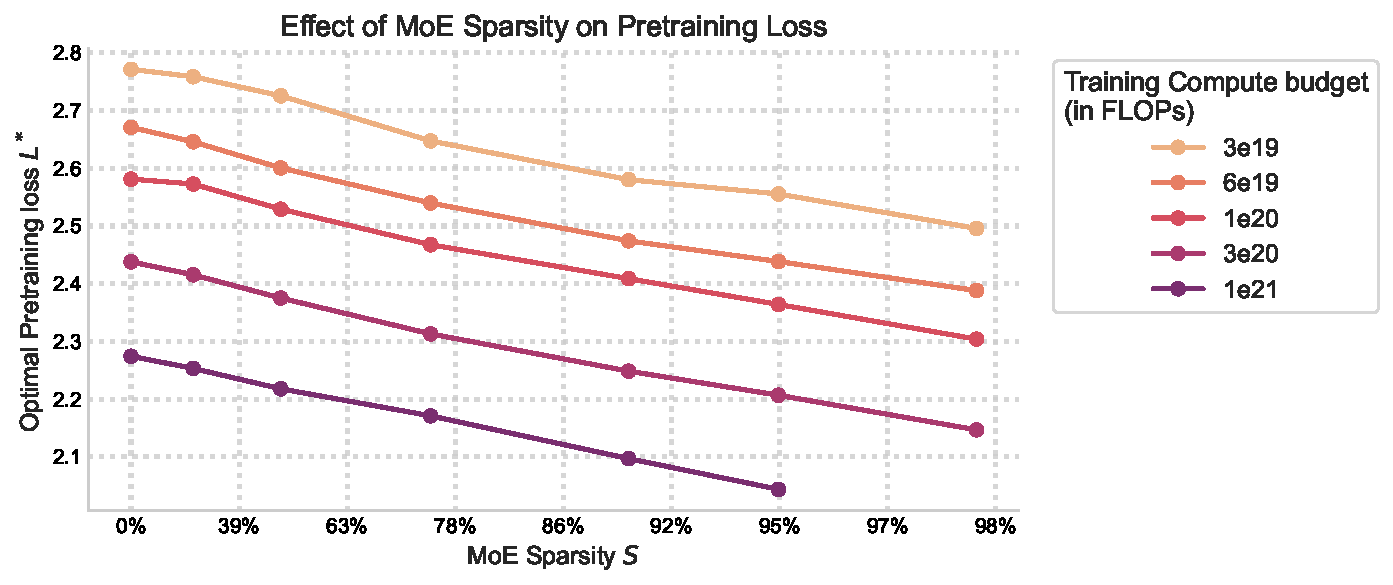
\includegraphics[width=0.7\textwidth]{plots/appendix/effect_of_sparsity_on_loss_thresholded.pdf}
    \caption{
    \textbf{Effect of \moe sparsity on pretraining loss across different training compute budgets}. 
    As sparsity increases, the validation loss decreases for all compute budgets, with larger budgets (darker lines) achieving lower losses at each sparsity level.
    This trend is consistent with the findings from~\Cref{sec:effect_of_training_budget}, demonstrating that increasing sparsity reduces the optimal pretraining loss across all compute budgets.
    % \todo[inline]{change this plot to log scale}
    % \Harshay{reminder to update plot if we decide to remove 1e21}
    % Notebook: \url{https://github.pie.apple.com/sabnar/l3m_core/blob/hs/notebooks/approach_2_sparsity_comparison.ipynb}
    }
    \label{fig:effect_of_sparsity_on_loss}
\end{figure}

\begin{figure}[tbp]
    \centering
    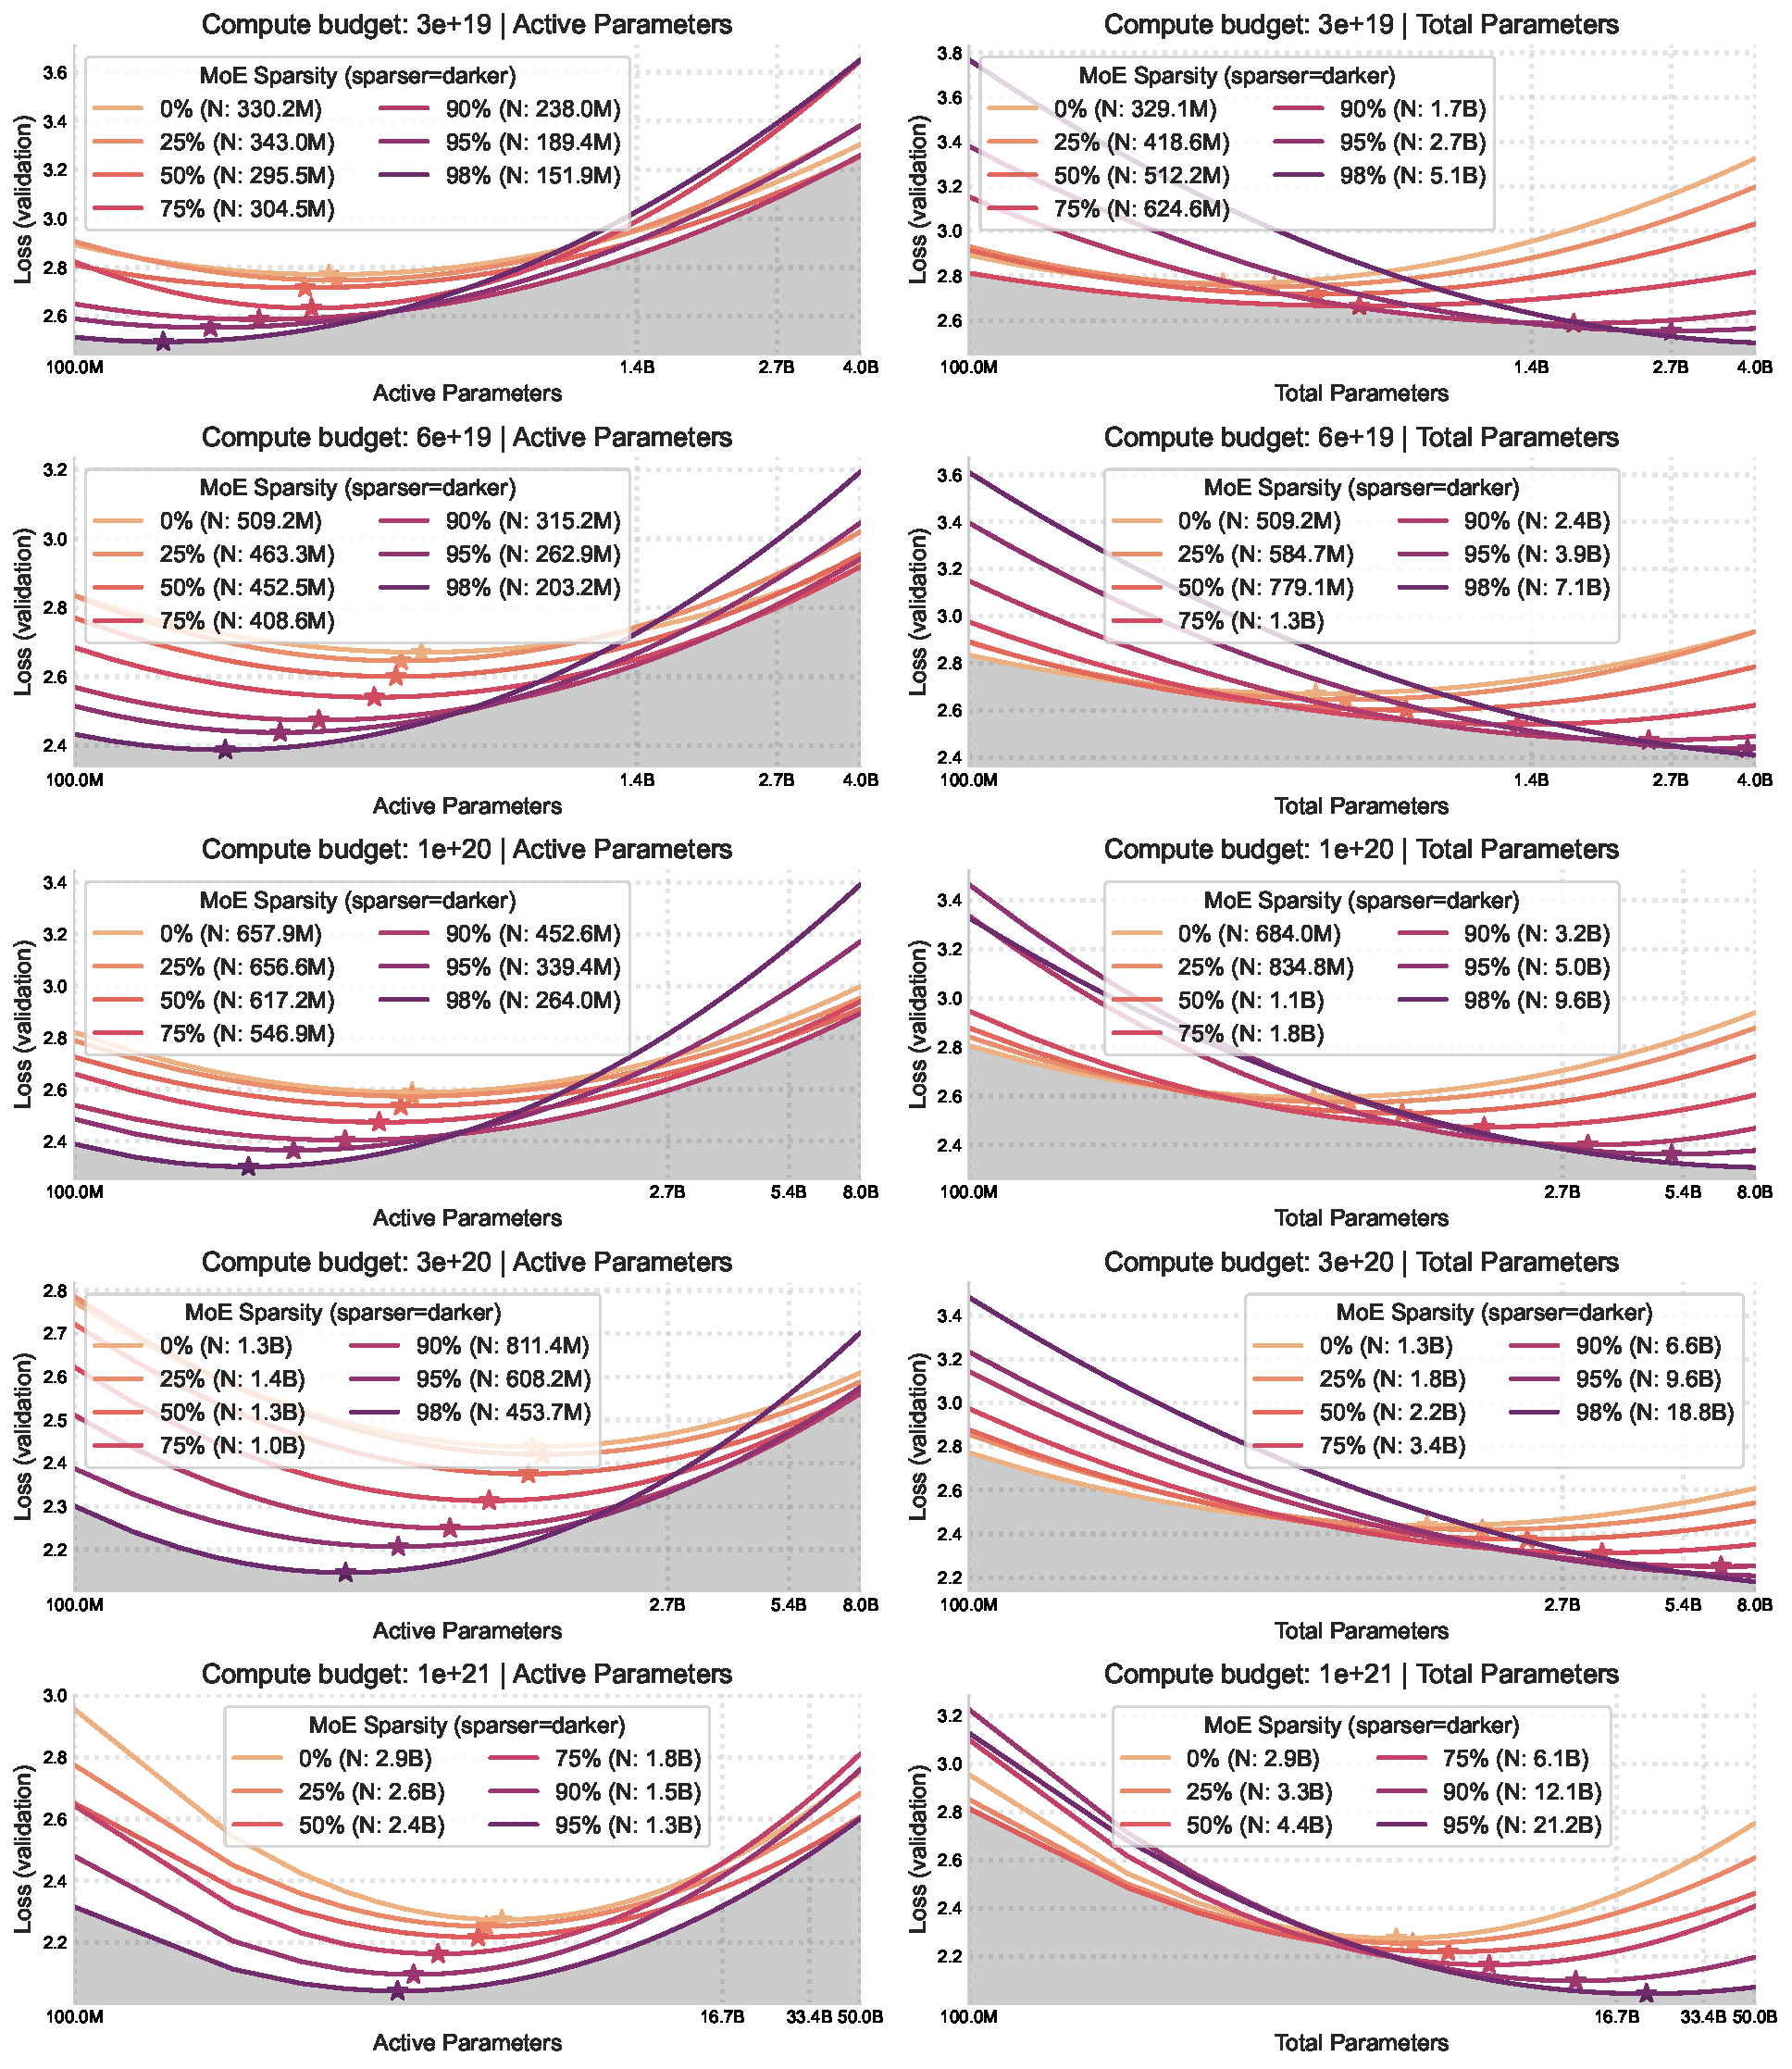
\includegraphics[width=0.8\textwidth]{plots/appendix/approach_2_sparsity_comparison_thresholded.pdf}
    \caption{
    \textbf{Effect of \moe sparsity on optimal total and active parameters across different training compute budgets.} 
    Each row shows the change in total and active parameters as a function of sparsity level for fixed training budgets. 
    Increasing sparsity leads to an increase in the optimal total parameters while reducing the optimal active parameters, consistent with our findings in~\Cref{sec:n_s_d_interaction} (\Cref{fig:iso_surface_sliced}). 
    Larger training compute budgets result in higher optimal (total and active) parameters across all sparsity levels.
    % \Harshay{reminder to update plot if we decide to remove 1e21}
    }
    \label{fig:chinchilla}
\end{figure}

